\documentclass[12pt, a4paper]{article}

\usepackage[hmargin=2.5cm, vmargin=2cm]{geometry}
\usepackage{amsthm, amssymb, mathtools, yhmath, graphicx}
\usepackage{fontspec, type1cm, titlesec, titling, fancyhdr, tabularx}
\usepackage{caption}
\usepackage{color}
\usepackage{hhline}
\usepackage{unicode-math}
\usepackage{nicefrac}
\usepackage{siunitx}
\usepackage{comment}

\usepackage[CheckSingle, CJKmath]{xeCJK}
\usepackage{CJKulem}
\usepackage{enumitem}
\usepackage[usenames, dvipsnames]{xcolor}
\usepackage{colortbl}
\usepackage{circuitikz}
%\setCJKmainfont[BoldFont=cwTex Q Hei]{cwTex Q Ming}
%\setCJKsansfont[BoldFont=cwTex Q Hei]{cwTex Q Ming}
%\setCJKmonofont[BoldFont=cwTex Q Hei]{cwTex Q Ming}
\setCJKmainfont[BoldFont=cwTeX Q Hei]{cwTeX Q Ming}

\def\normalsize{\fontsize{12}{18}\selectfont}
\def\large{\fontsize{14}{21}\selectfont}
\def\Large{\fontsize{16}{24}\selectfont}
\def\LARGE{\fontsize{18}{27}\selectfont}
\def\Huge{\fontsize{20}{30}\selectfont}

\titleformat{\section}{\bf\Large}{\arabic{section}}{24pt}{}
\titleformat{\subsection}{\large}{\arabic{subsection}.}{12pt}{}
\titlespacing*{\subsection}{0pt}{0pt}{1.5ex}

\parindent=24pt

\DeclarePairedDelimiter{\abs}{\lvert}{\rvert}
\DeclarePairedDelimiter{\norm}{\lVert}{\rVert}
\DeclarePairedDelimiter{\inpd}{\langle}{\rangle}
\DeclarePairedDelimiter{\ceil}{\lceil}{\rceil}
\DeclarePairedDelimiter{\floor}{\lfloor}{\rfloor}

\newcommand{\unit}[1]{\:(\text{#1})}
\newcommand{\img}{\mathrm{i}}
\newcommand{\mD}{\mathrm{d}}

\title{ \bf {\huge 電子電路實驗5:RC與RL電路之步級響應}\\ 實驗結報}
\author{B02901178 江誠敏}
\date{2014/09/21}

\begin{document}

\maketitle

\section{實驗目的}
步級響應(step response)在線性系統中是一項非常有用的特性,本實驗將研究一次線性電路(first-order circuit),即常見的 RC、RL 電路的步級響應。
\section{實驗步驟}
\begin{enumerate}[itemsep=0pt]
  \item 利用LCR計,記錄所使用的各個電容以及電感的確實量值;利用電表記錄固定電阻的量值。
  \item 連接電路如下圖,其中C = 0.1,R為10 可變電阻,V為低電位差−5, 高電位差5V,頻率 500Hz 之方波。
  \item 使用示波器觀察在不同電阻值時 vC及 vR的波形,並記錄方波電位由−5V 變為 5V 與 vC
    電位達到 1.32V 的時間差。
  \item 連接電路如圖,其中 L =10 mH,R 為 5kΩ 可變電阻,v 為低電位差−5V, 高電位差
    5V,頻率 50kHz 之方波。
  \item 使用示波器觀察在不同電阻值時 vL及 vR的波形,並記錄方波電位由−5V 變為 5V 與 vR
    電位達到 1.32V 的時間差。
\end{enumerate}


  \begin{center}
    \begin{tikzpicture}[american voltages, scale=0.8]
      \draw[color=black, thick]
      (0, 0) to [V=$V_S$] (0, 6) 
      (0, 6) to [R, l=$R$] (6, 6) 
      (6, 6) to [C, v=$V_C$] (6, 0)
      (6, 0) to [short] (0, 0)
      (3, 0) node[ground]{}
      ;
    \end{tikzpicture}
    \quad
    \begin{tikzpicture}[american voltages, scale=0.8]
      \draw[color=black, thick]
      (0, 0) to [V=$V_S$] (0, 6) 
      (0, 6) to [R, l=$R$] (6, 6) 
      (6, 6) to [L, v=$V_L$] (6, 0)
      (6, 0) to [short] (0, 0)
      (3, 0) node[ground]{}
      ;
    \end{tikzpicture}
  \end{center}


  \section{預報問題}

  \begin{enumerate}[itemsep=20pt, topsep=10pt]
    \item {\large 請推導實驗中使用的一次電路步級響應的理論值(二個圖都要推導)。} \\[10pt]
      由 Kirchhoff's circuit laws有
      \[
        V_S - iR - \frac{q}{C} = 0 
      \]
      由上式可以得出一個關於$q$的微分方程
      \[
        V_S - R\frac{ \mD q }{ \mD t} - \frac{q}{C} = 0 
      \]
      此微分方程的解為
      \[
        q = V_S C \left( 1 + c \mathrm{e}^{-t/RC} \right) 
      \]
      其中$c$為一待定常數。注意到在上一個週期,電容已經被充電成端電壓為$-V_S$,因此
      \[
        -V_S C = q(0) = V_S C ( 1 + c )
      \]
      因此可知
      \[
        c = -2
      \]
      從而我們可以得知電容的端電壓為
      \[
        V_C = V_S \left( 1 - 2 \mathrm{e}^{-t/RC} \right)
      \]
      電感的情況類似,由 Kirchhoff's circuit laws有
      \[
        V_S - \frac{\mD i}{\mD t}R - i R = 0 
      \]
      此微分方程的解為
      \[
        i = \frac{V_S}{R} \left( 1 + c \mathrm{e}^{-Rt/L} \right) 
      \]
      其中$c$為一待定常數。注意到在上一個週期末時,電流為$-\frac{V_S}{R}$,而電流必需連續,否則電感的電壓會到無限大。
      因此$c = -2$
      \[
        i = \frac{V_S}{R} \left( 1 - 2 \mathrm{e}^{-Rt/L} \right) 
      \]
      \[
        V_L = 2 V_S \mathrm{e}^{-Rt/L} 
      \]
    \item {\large 請使用 PSpice 或者其他電路模擬軟體模擬實驗中使用的一次電路。} \\[10pt]

      \begin{itemize}
        \item RC電路
      \begin{center}
        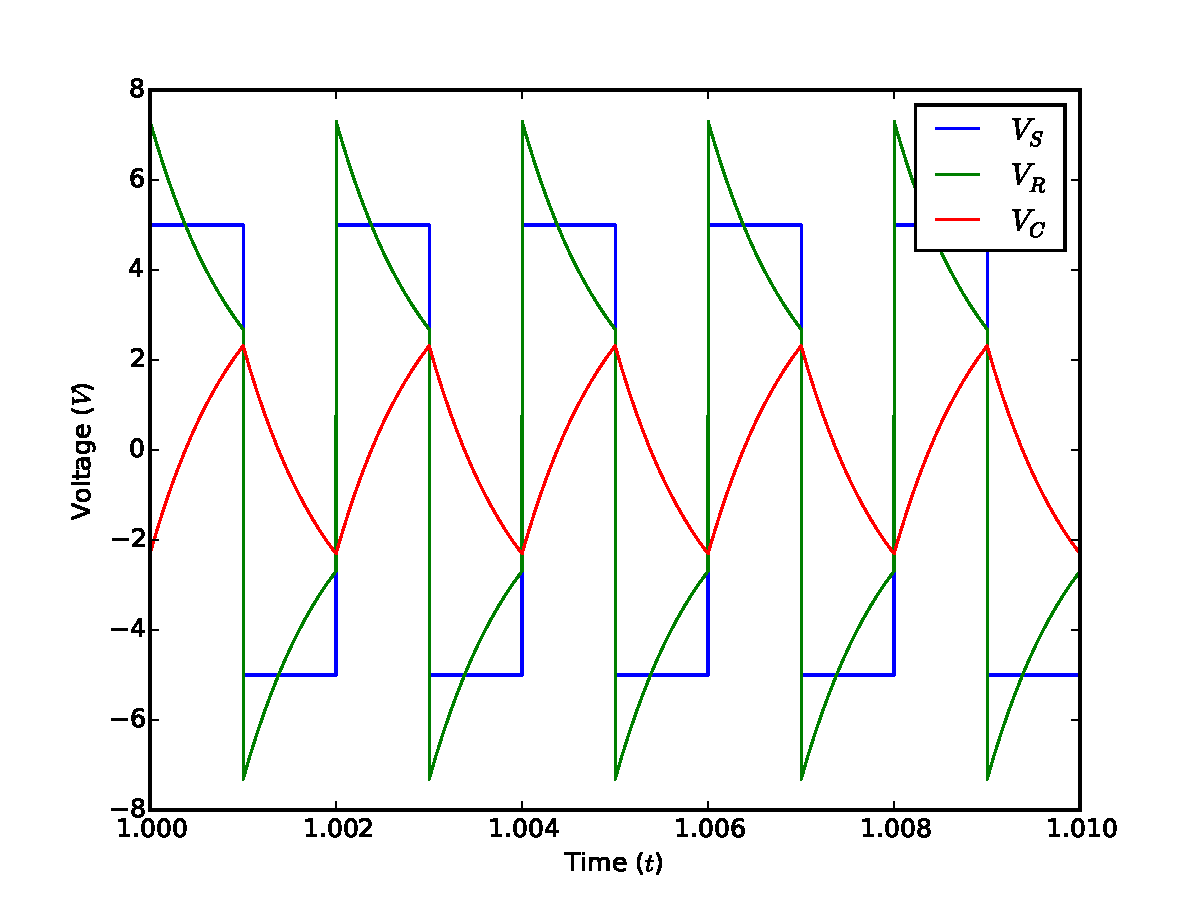
\includegraphics[width=0.6\textwidth]{plt1.pdf}
      \end{center}
        \item RL電路
      \begin{center}
        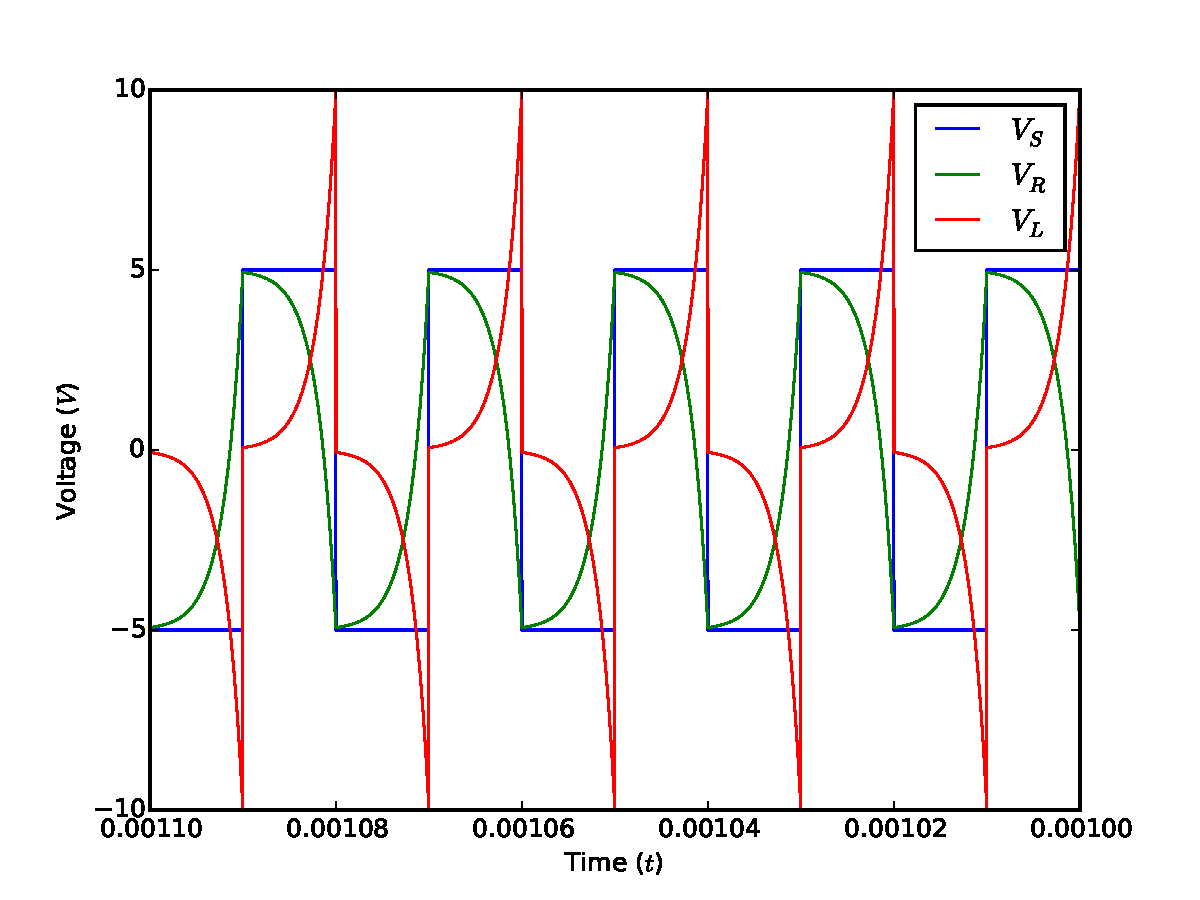
\includegraphics[width=0.6\textwidth]{plt2.pdf}
      \end{center}
  \end{itemize}
  
  \end{enumerate}

\end{document}


